% ============================================================================
% AntMill full paper draft (v0.1, 2026-07-12)
% TODO before AAAI-27 submission: swap to aaai27.sty two-column format,
% anonymize, move draft-status box to a footnote or delete, check page limit.
% Compile: pdflatex -> bibtex -> pdflatex -> pdflatex
% ============================================================================
\documentclass[11pt]{article}

\usepackage[margin=1in]{geometry}
\usepackage{booktabs}
\usepackage{graphicx}
\usepackage{amsmath}
\usepackage[hidelinks]{hyperref}
\usepackage{xcolor}
\usepackage{enumitem}
\usepackage{microtype}
\usepackage{siunitx}
\usepackage[numbers,sort&compress]{natbib}

\graphicspath{{figures/beta/}{figures/}}

\title{Locally Plausible, Globally Wasteful:\\ Consensus Consolidation of Shared Experience\\ Silently Degrades Multi-Agent LLM Systems}
\author{Anonymous submission}
\date{Draft v0.1 --- \today}

\begin{document}
\maketitle

\begin{center}
\fcolorbox{teal!70!black}{teal!5}{\parbox{0.94\linewidth}{%
\textbf{Draft status.} All confirmatory numbers come from preregistered protocols
(\texttt{prereg\_phase\_beta.md}, \texttt{prereg\_phase\_gamma.md} and its frozen appendices);
gate rules were frozen before data collection and every verdict, deviation, and negative result
is recorded in the corresponding deviation or decision log. Statistics are same-task paired
bootstrap (10{,}000 resamples, 95\% CI) with per-seed sign tables. Experience text is entirely
model-generated; a sanitizer guarantees no researcher-authored string enters any memory pool.
\textbf{TODO}: P3 (MiniWoB task generalization, rerun under amendment 01) pending; integrate
when the frozen gate reports.}}
\end{center}

\begin{abstract}
Multi-agent LLM systems increasingly share experiential memory: agents write distilled insights
into a common pool that is retrieved and injected into every teammate's context. We study a
failure mode of this design that does not require wrong facts, poisoned text, or illegal
actions. In a controlled trap-maze microscope where every route is legal and shortest-path cost
is exactly measurable, we run a preregistered ladder of experiments over faithful
instantiations of published components (ExpeL-style insight operations, Generative-Agents-style
retrieval). We find that (i) single-agent faithful experience learning leaves primary
efficiency endpoints unchanged (an attribution control); (ii) across a five-arm multi-agent
matrix, actively injected memory degrades efficiency and amplifies looping, and
\emph{consensus-consolidated} shared memory is the most reproducibly harmful arm
(success-only excess steps $+11.8$, CI $[7.7, 16.0]$; loop rate $+0.138$, CI $[0.092, 0.188]$;
$5/5$ seeds), the only arm whose loop amplification significantly exceeds private memory;
(iii) the harm is not read-side usage-weighted retrieval (a preregistered null dose-response)
and persists without self-healing over a $T{=}10$ horizon, while the append protocol
\emph{improves} over the same horizon; (iv) a write-side audit shows consolidation compresses
the population's active strategy supply by ${\sim}2.3\times$. Two preregistered rescue
interventions constrain the mechanism's causal status: naively re-exposing consolidated-away
variants at added dose fails and worsens stagnation, and an equal-dose archive is unreachable
under fixed-capacity similarity retrieval---the cheapest ``keep the deleted memories'' fix does
not work. A cross-model probe (Qwen3-32B) structurally replicates the supply compression but
leaves the efficiency effect unresolved and excludes a loop amplification of the primary
model's magnitude, bounding the phenomenon's transfer. We release the microscope, all
preregistrations, and per-route artifacts.
\end{abstract}

% ============================================================================
\section{Introduction}
% ============================================================================

When army ants lose the pheromone trail, each ant follows the locally impeccable rule
``follow the ant in front of you,'' and the colony organizes itself into a circular mill that
marches until exhaustion. No single step is wrong; the composition is fatal.

We present evidence that shared experiential memory in multi-agent LLM systems admits an
analogous failure. The prevailing design pattern---popularized for single agents by
experiential learners such as ExpeL~\citep{zhao2024expel} and Reflexion~\citep{shinn2023reflexion},
and extended to agent teams by experiential co-learning~\citep{qian2024colearning} and
cross-task multi-agent experience pools~\citep{liu2025mael}---lets agents distill natural-language
insights from their own trajectories, store them in a memory pool, and retrieve them as guidance.
When the pool is \emph{shared} and a reviewer LLM \emph{consolidates} it by consensus
(merging, editing, up/down-voting insights), every ingredient is individually reasonable and
individually published. The composition, we show, is not.

The failure we characterize is \emph{silent}. Agents keep succeeding, never cross walls, never
submit false answers; the experience text is locally plausible and derived from genuine
trajectories. Yet routes grow longer, agents revisit the same cells, and loop signatures rise
--- and the effect intensifies exactly under the write protocol that is supposed to improve
memory quality. Because no error is ever emitted, standard success-rate dashboards do not see
it.

Studying such a compositional failure on a live benchmark confounds every knob at once. We
instead build a \emph{mechanism microscope}: a generated $15\times15$ trap-maze family with
known shortest paths, local observations, and a step cap, in which efficiency loss and looping
are exactly measurable per route. Into this microscope we place faithful instantiations of
published components (Table~\ref{tab:components}), so that any degradation is attributable to
the composition---sharing and consolidation---rather than to home-made machinery. All
confirmatory experiments were preregistered with frozen gates; every deviation and negative
result appears in an append-only log.

\paragraph{Contributions.}
\begin{enumerate}[leftmargin=1.6em]
\item \textbf{A preregistered phenomenon.} In a five-arm multi-agent memory matrix over five
seeds, consensus-consolidated shared memory degrades success-only route efficiency
($+11.8$ excess steps, CI $[7.7,16.0]$), amplifies loops ($+0.138$, CI $[0.092,0.188]$), and
reduces success ($-0.171$), relative to a write-only frozen control; storage alone is harmless
and multi-agent execution alone is not pathological. Relative to \emph{private} memory, the
shared-specific risk is loop amplification ($+0.058$, CI $[0.008,0.113]$), not a broad
efficiency gap (Section~\ref{sec:beta}).
\item \textbf{Locating the channel.} A preregistered read-side dose-response is null, while a
write-side audit shows consolidation compresses the population's active strategy supply
${\sim}2.3\times$ (11.0 vs.\ 25.4 distinct injected experiences). Over $T{=}10$ the harm
persists without self-healing while the uncompressed append protocol significantly
self-improves (Section~\ref{sec:beta}).
\item \textbf{Intervention boundaries.} Two preregistered archive-rescue interventions show
that the obvious mitigation---keep consolidated-away variants retrievable---fails: at added
dose it worsens stagnation ($+0.045$, CI $[0.023,0.067]$); at equal dose the archive is
unreachable because consolidated insights dominate the similarity ranking. Supply compression
therefore remains a robust \emph{correlate} whose causal status is honestly unresolved
(Section~\ref{sec:gamma}).
\item \textbf{Transfer bounds.} A cross-model probe on Qwen3-32B structurally replicates the
write-side compression (1.55$\times$ vs.\ 1.68$\times$ at matched horizon) but not the
behavioral coupling: the efficiency endpoint is direction-consistent yet underpowered, and a
loop amplification of the primary model's magnitude is excluded (Section~\ref{sec:gamma}).
\item \textbf{A reusable microscope and discipline.} We release the environment, runners,
paired-bootstrap statistics, sanitizer, memory audits, preregistrations with freeze hashes, and
per-route artifacts (Section~\ref{sec:method}).
\end{enumerate}

% ============================================================================
\section{Related Work}
% ============================================================================

\paragraph{Single-agent experiential learning.} ExpeL~\citep{zhao2024expel} distills insights
from success/failure trajectories with ADD/EDIT/UPVOTE/DOWNVOTE operations and retrieves them
as guidance; Reflexion~\citep{shinn2023reflexion} converts failures into verbal
self-corrections; ReAct~\citep{yao2023react} interleaves reasoning and acting;
Generative Agents~\citep{park2023generative} score memories by relevance, importance, and
recency; MemoryBank~\citep{zhong2024memorybank} adds long-term memory management. These works
established that experience helps a \emph{single} agent. Our write operations, retrieval
scoring, and distillation prompts are faithful reimplementations of this line
(Table~\ref{tab:components}); we stress-test their composition, not their original claims.

\paragraph{Multi-agent experience sharing.} Experiential
co-learning~\citep{qian2024colearning} shares shortcut experiences between instructor and
assistant agents in ChatDev~\citep{qian2024chatdev}; MAEL~\citep{liu2025mael} equips each agent
in a collaboration graph with an experience pool queried by similarity and reward;
multi-agent debate~\citep{du2024debate} and self-consistency~\citep{wang2023selfconsistency}
aggregate opinions rather than memories; MetaGPT~\citep{hong2024metagpt} shares a message pool.
All published sharing designs accumulate experience additively. To our knowledge, no prior
work evaluates the natural next step---\emph{LLM-driven consensus consolidation of a shared
experience pool}---as an intervention with controls; that protocol is exactly our subject.

\paragraph{Memory risk and governance.} A concurrent 2026 line studies shared-memory
governance: failure taxonomies for multi-tenant memory~\citep{governed2026sharedmem},
stress-tests of memory systems~\citep{memfail2026}, drift and poisoning
risks~\citep{ssgm2026}, and longitudinal safety risks of memory-equipped
agents~\citep{remembering2026}. These works propose frameworks and taxonomies over deployed
or synthetic traces. We complement them with a preregistered, controlled, intervention-bearing
study of one specific mechanism---consolidation-induced degradation---with exact route-level
ground truth, and with negative results that bound the cheapest mitigation.

% ============================================================================
\section{The Maze Microscope}\label{sec:method}
% ============================================================================

\paragraph{Environment.} We generate a $15\times15$ ``trap'' maze family with enforced
shortest-path length $\geq 30$ and disjoint train/heldout splits per experiment seed. Solvers
receive local observations only (no maze graph, no shortest path), act under a 120-step cap,
and are scored by exact excess steps over the known optimum. Efficiency loss and loop
signatures are therefore measurable per route---the property that makes silent degradation
visible at all.

\paragraph{System under test.} Four solver agents attempt the \emph{same} tasks in independent
environment copies. They never communicate and never vote; the \emph{only} coupling channel is
the experience memory, so any cross-agent effect is attributable to it. Each round $t$
comprises (i) evaluation on 12 heldout mazes per agent (48 routes), (ii) a training batch of
4 mazes per agent (16 routes), and (iii) a reviewer LLM that sees only logs and quality
signals---never hidden routes---and writes to the memory pool under the arm's protocol. The
final round evaluates without writing. Retrieval injects the top-$k{=}6$ insights
(Generative-Agents scoring; $\lambda{=}0$ outside the dose-response experiment) into the solver
prompt; the pool is capped at 80.

\begin{table}[t]
\centering
\caption{Every component is a faithful instantiation of a published method; only the
composition (shared pool + consensus consolidation) is new, and it is the subject of study.}
\label{tab:components}
\begin{tabular}{ll}
\toprule
Component in our system & Source \\
\midrule
Insight ops ADD/EDIT/UPVOTE/DOWNVOTE, importance-0 deletion & ExpeL~\citep{zhao2024expel} \\
Retrieval scoring (relevance + importance + recency, $\lambda$) & Generative Agents~\citep{park2023generative} \\
Insight distillation from success/failure trajectories & ExpeL~\citep{zhao2024expel} \\
Stepwise solving with injected experience & ReAct-style~\citep{yao2023react} \\
Shared pool across agents & Co-learning line~\citep{qian2024colearning,liu2025mael} \\
Consensus consolidation of the shared pool & \textbf{composition under test} \\
\bottomrule
\end{tabular}
\end{table}

\paragraph{Arms.} The five-arm matrix decomposes ``multi-agent shared consolidated memory''
factor by factor: \texttt{no-memory} (is multi-agent execution itself pathological?);
\texttt{frozen} (reviewer writes, solvers never read: is \emph{storage} harmful?);
\texttt{private} (per-agent pools: is \emph{sharing} necessary?); \texttt{shared-append}
(shared but never merged: is sharing \emph{without} consolidation harmful?); and
\texttt{shared-consolidated} (the pattern under indictment).

\paragraph{Endpoints and statistics.} Primary preregistered endpoints: success-only excess
steps, loop rate, and the multi-agent ant-mill rate (loop + route overlap). Auxiliary:
success, stagnation, maximum revisits, cost ratio, route diversity. Mechanism audit (logged
per run): pool-size trajectory, \emph{distinct injected experiences}, retrieval entropy and
top-1 share, sanitizer rejections, LLM errors. All verdicts use same-maze same-agent paired
bootstrap (10k resamples, 95\% CI) and must be accompanied by per-seed sign tables. A
sanitizer rejects maze IDs, coordinates, and fixed action sequences from memory text; cache
keys are salted by (run, seed, round, task, agent, step). The primary model is
DeepSeek-V3~\citep{deepseek2024v3} via a fixed endpoint; a preregistered drift probe (cache
disabled, replaying a frozen-arm round) verified distributional stability before any reuse of
cached controls.

% ============================================================================
\section{Preregistered Results: the Phenomenon}\label{sec:beta}
% ============================================================================

\subsection{E1: single-agent attribution control}

Before introducing sharing, we ask whether faithful experience learning changes single-agent
behavior at all. Relative to a no-memory baseline (paired, final round, three seeds), neither
the ExpeL-operations writer nor the append writer moves any primary endpoint: success-only
excess steps CIs contain zero (append $-4.74$, CI $[-14.1, +4.2]$; ops $+5.11$, CI
$[-6.4, +16.3]$), as do loop rates. By the frozen rule this is a \textbf{FAIL}, recorded as
such. However, the mandated adherence analysis shows experience is \emph{not} ignored: the ops
writer shifts action selection away from the controller suggestion after memory activates
($+0.041$ deviation, same sign in $3/3$ seeds), and the append writer significantly reduces
maximum revisits. The single-agent null is therefore an \emph{attribution control}: any
multi-agent degradation cannot be attributed to ``using memory'' per se, only to the sharing
channel.

\subsection{E2: multi-agent memory matrix}

We compare the five arms at four agents, $T{=}6$, five seeds, against the write-only
\emph{frozen} control. Table~\ref{tab:e2} and Figure~\ref{fig:fig2} report paired differences
at the final round.

\begin{table}[h]
\centering
\caption{E2 final-round paired differences versus frozen write-only memory (five seeds,
$n_{\text{pairs}}=240$; success-only excess steps drops unpaired failures).
$^\ast$ = 95\% CI excludes zero.}
\label{tab:e2}
\begin{tabular}{lrrrr}
\toprule
Arm & Success & Success excess steps & Loop rate & Max revisits \\
\midrule
MAS no memory      & $-0.004$          & $+1.12$            & $+0.042^\ast$ & $+0.10$ \\
Private memory     & $-0.175^\ast$     & $+7.32^\ast$       & $+0.079^\ast$ & $+1.20^\ast$ \\
Shared append      & $-0.121^\ast$     & $+2.75$            & $+0.025$      & $+0.23$ \\
Shared consolidated& $-0.171^\ast$     & $+11.84^\ast$      & $+0.138^\ast$ & $+1.68^\ast$ \\
\bottomrule
\end{tabular}
\end{table}

Three readings follow. First, multi-agent execution is not itself pathological: MAS-no-memory
matches frozen on efficiency and success, with only a small loop increase ($+0.042$,
CI $[0.008, 0.075]$); frozen itself matches no-memory, so \emph{storage is harmless and
injection is the harm channel}. Second, \textbf{consensus-consolidated shared memory meets
every preregistered degradation criterion}: success-only excess steps $+11.84$
(CI $[7.66, 16.02]$), same-sign in $5/5$ seeds and \emph{larger} in the later seeds; loop rate
$+0.138$ (CI $[0.092, 0.188]$); success $-0.171$. Third, the broad risk is active injection
rather than sharing alone---private memory also degrades---so we test the sharing-specific
claim directly.

\paragraph{Shared versus private boundary.} Figure~\ref{fig:fig2b} contrasts the shared arms
against a \emph{private} baseline. The efficiency separation is not significant (consolidated
vs private success-only excess steps $+0.87$, CI $[-4.29, +6.15]$), but loop amplification is:
consolidated loops significantly more than private ($+0.058$, CI $[0.008, 0.113]$), while
append loops \emph{less}. The honest claim is therefore that consensus consolidation
specifically amplifies looping relative to private memory; we do not claim a broad
shared-over-private efficiency gap.

\subsection{E3: read-side dose-response is null}

If the harm were read-side---agents increasingly retrieving a few high-vote memories---then
raising the importance weight $\lambda$ in Generative-Agents-style scoring should deepen
degradation. It does not. Sweeping $\lambda\in\{0,0.5,1\}$ on the append arm (three seeds,
$T{=}6$), the paired difference of $\lambda{=}1$ versus $\lambda{=}0$ on success-only excess
steps is $+1.69$ (CI $[-4.26, +7.61]$), loop rate $+0.049$ (CI $[0.000, 0.104]$), and
final-round retrieval entropy is non-monotone in $\lambda$ ($0.833/0.826/0.845$). The
read-side usage-weighted-feedback hypothesis is \textbf{refuted}; we report it as a clean null.

\subsection{Mechanism audit: write-side strategy-supply compression}

An offline audit of the same E2 runs locates the concentration on the \emph{write} side
(Figure~\ref{fig:fig3}). Under identical settings, the consolidated pool converges to
$14.2$ items with only $11.0$ distinct experiences ever injected across all rounds, whereas
the append pool grows to the cap ($80$) and injects $25.4$ distinct experiences, and private
injects $37.6$. Consensus consolidation compresses the population's active strategy supply by
roughly $2.3\times$ relative to append. The top-1 retrieval share rises in step, but this is a
consequence of the smaller pool rather than an independent channel; the load-bearing evidence
is the direct pool-size and distinct-injection counts. Given the intervention results of
Section~\ref{sec:gamma}, we report compression as a robust, cross-checked \emph{correlate} and
candidate mechanism, not as established cause.

\subsection{E4: long-horizon stress test (exploratory)}

To ask whether the write-side harm saturates, deepens, or self-heals over a longer feedback
horizon, we extend the four-agent shared arms to $T{=}10$ (three seeds, heldout 12, frozen and
shared-append included as controls; not gate-bound, per the preregistration). Relative to
frozen, shared-consolidated's degradation is present at every checkpoint we tested
($t=3,6,9$) and does not narrow: success drops $-0.174$, $-0.146$, $-0.257$ (all CIs exclude
zero), and loop rate rises $+0.083$, $+0.083$, $+0.118$ (all CIs exclude zero), with the final
round the worst of the three. A stricter within-condition test---comparing each condition's own
last three rounds to its first three (excluding the warm-up round $t{=}0$)---finds no
significant self-trend for shared-consolidated on any of six endpoints: the gap opens early
and persists at a noisy plateau rather than provably deepening. The append arm, in contrast,
shows a significant within-condition \emph{improvement} over the same horizon (cost ratio
$-0.079$, excess steps $-3.50$, stagnation $-0.026$, max revisits $-0.340$, all CIs exclude
zero) and by $t{=}9$ is significantly cheaper than frozen on cost ratio, excess steps, and max
revisits---consistent with a write protocol whose strategy supply is not compressed continuing
to benefit from accumulation. This contrast is also the paper's validity anchor: the same
read/write infrastructure that degrades under consolidation \emph{helps} under append, so the
harm cannot be blamed on ``memory'' or on our plumbing. Per-seed decomposition exposes
heterogeneity the pooled estimate hides: seed 1 is the only seed with a significant
late-vs-early decline in success ($-0.097$, CI excludes zero); seed 2 has the most severe
round-wise trajectory, ending at success $0.17$ and loop rate $0.46$, though its late-vs-early
CI includes zero; seed 0 shows no significant decline. The pooled ``no significant further
drift'' verdict is a mean over a mixed population, not evidence that every instance is equally
stable.

\subsection{The failure is silent}

Figure~\ref{fig:fig1} shows the mechanism schematic and a case study mined from the runs: the
same held-out maze and agent at the final round, whose shortest path is 38 steps. As the write
protocol consolidates, the route degrades monotonically---frozen 39 steps (one revisit),
private 47 (four), shared-append 55 (nine), shared-consolidated 73 with cost 1.92, eleven
revisits to the same cell, and a detected loop---yet every route is legal and every arm still
reaches the goal. This is the ant-mill signature: not a false belief, but a locally plausible
correction signal, reinforced through consensus writing, that composes into a globally
wasteful cycle.

% ============================================================================
\section{Mechanism Interventions and Boundaries}\label{sec:gamma}
% ============================================================================

Phase Gamma preregistered three short, gated extensions: two archive-rescue interventions on
the primary model, and a cross-model probe. All gates, thresholds, and interpretation branches
were frozen before data; a drift probe (frozen-arm round replayed with cache disabled; all four
probe metrics inside the original bootstrap CIs) authorized reuse of the cached E2 controls.

\subsection{Rescue I: additive archive access fails and backfires}

The cheapest conceivable mitigation is to make consolidation non-destructive: retain
DOWNVOTE-deleted insights, pre-edit versions, and similarity-merge-discarded variants in a
read-only \emph{archive} that solvers can still retrieve. Our first preregistered rescue arm
implemented archive access additively (active top-6 \emph{plus} archive top-6), which doubles
the injected dose to 12 items per prompt---a deviation we record and exploit. The manipulation
itself succeeded: distinct injected experiences roughly doubled (21/21/27 vs.\ 12/11/14 in the
matched E2 consolidated seeds), with archive items winning about half the retrieval slots. The
behavior did not improve on a single endpoint. Success non-inferiority failed
($-0.056$, CI $[-0.153, +0.042]$ against a $-0.05$ bound); success-only excess steps were null
($-0.45$, CI $[-6.86, +5.96]$); loops trended \emph{worse} ($+0.035$); and stagnation
significantly worsened ($+0.045$, CI $[+0.023, +0.067]$). Read as a designed-fix evaluation:
\textbf{naively re-exposing the material consolidation discarded, at added dose, does not
rescue behavior and aggravates stagnation}---consistent with E2's finding that injection
itself is the harm channel.

\subsection{Rescue II: the equal-dose archive is unreachable}

The confounded dose motivated a second, clean arm: one \emph{joint} ranking over active pool
and archive with the original total top-6, leaving the per-prompt dose identical to E2. The
preregistered manipulation check required the cumulative distinct injected supply to expand by
$\geq 1.5\times$ in at least $2/3$ seeds. It did not (ratios $1.42/1.55/1.07$), and not
because the archive was ignored---archive items appeared in $896/912$ retrievals where
candidates existed. Under a fixed retrieval capacity, consolidated insights dominate the
similarity ranking, so the archive cannot expand \emph{diversity}, only substitute items. Per
the frozen amendment, the behavioral gate was therefore not evaluated
(\texttt{not\_evaluable}), and we explicitly do \emph{not} claim that equal-dose archive rescue
is ineffective. The constructive reading: \textbf{the popular ``never really delete; keep an
archive'' design does not restore strategy diversity under fixed-capacity similarity
retrieval}---a reachability bottleneck any governance proposal must confront.

Together the two rescue arms leave strategy-supply compression as a strong correlate whose
causal role is unresolved: the additive test was dose-confounded by design accident, and the
clean test could not move the mediator. We report this plainly rather than promoting the
mechanism to a causal claim.

\subsection{Cross-model probe: compression replicates, coupling does not}

We repeated the frozen/append/consolidated triangle on Qwen3-32B~\citep{yang2025qwen3}
(three seeds, $T{=}4$, justified by E4's finding that the primary-model gap is established by
$t{=}3$; thinking mode disabled after a passing calibration smoke: 100\% action parse rate,
baseline success 0.479). The preregistered gate reports
\texttt{not\_detected\_or\_underpowered}, but the three endpoints earn three different honest
readings:

\begin{itemize}[leftmargin=1.6em]
\item \emph{Efficiency: unresolved, direction-consistent.} Success-only excess steps
$+5.83$ with all three seeds positive ($+12.4/+0.9/+1.8$), but CI $[-3.75, +15.20]$
($n{=}40$ success pairs) contains both zero \emph{and} the DeepSeek effect ($+11.84$): the
probe cannot adjudicate between no effect and a full-size effect. Power was consumed by
Qwen's lower baseline success, which shrinks the success-only pair count.
\item \emph{Loops: a bounded difference.} Loop rate $-0.076$, CI $[-0.153, 0.000]$: the CI
\emph{excludes} the primary model's $+0.138$. A loop amplification of that magnitude is
absent on Qwen at these settings. We report this as an exploratory magnitude comparison, not
as a preregistered boundary claim.
\item \emph{Success: no drop.} $+0.042$, CI $[-0.049, +0.132]$, excluding the primary model's
$-0.171$; consolidated memory neither helps nor measurably harms success on Qwen.
\end{itemize}

Crucially, the \emph{mechanism precondition} does transfer: at the matched horizon
($t{=}3$), consolidation compresses the distinct injected supply on Qwen by $1.55\times$
(13.3 vs.\ 20.7) versus $1.68\times$ on DeepSeek---nearly identical compression, different
behavioral coupling. Structural compression without detected harm on one model further
cautions against treating compression alone as a sufficient cause, and is exactly consistent
with the rescue results above.

% P3 (MiniWoB task generalization) is rerunning under prereg amendment 01 after an
% action-interface repair (bid-visible observations + semantic execution calibration).
% TODO: integrate the frozen gate report here; the paper's claims do not depend on it.

% ============================================================================
\section{Design Implications}
% ============================================================================

\begin{enumerate}[leftmargin=1.6em]
\item \textbf{Do not consensus-consolidate shared experience by default.} The same
infrastructure that degrades under consolidation improves under append-and-retrieve (E4's
significant within-condition gains). If dedup or cap pressure demands consolidation, treat it
as a risk surface, not hygiene.
\item \textbf{Monitor the write side, not just success.} Distinct injected experiences,
pool-size trajectory, and retrieval concentration are cheap, logged-at-source early-warning
signals; success-rate dashboards are blind to silent efficiency decay by construction.
\item \textbf{Loop and stagnation signatures belong in agent telemetry.} Repeated
state-action signatures and stagnation rate separated consolidated from private memory when
aggregate efficiency could not.
\item \textbf{``Keep an archive'' is not a free fix.} At added dose it backfires; at equal
dose fixed-capacity similarity retrieval never reaches the archive. Governance proposals that
retain pruned memories must also change the \emph{reachability} of what they retain.
\end{enumerate}

% ============================================================================
\section{Limitations}
% ============================================================================

Our confirmatory evidence is single-environment and single-model-family: a controlled maze
microscope on DeepSeek-V3, chosen because its difficulty band makes silent degradation exactly
measurable and because cheap open models are precisely what shared-memory multi-agent
deployments run in practice; the precedent for mid-tier backbones in this literature is
explicit~\citep{zhao2024expel}. The cross-model probe bounds but does not establish transfer:
efficiency is unresolved (underpowered), and the loop signature does not carry at the primary
model's magnitude. The compression mechanism remains a candidate---our own interventions
constrain it honestly. Task-family generalization (MiniWoB~\citep{shi2017wob,liu2018miniwob}
via BrowserGym~\citep{chezelles2024browsergym}) is preregistered and in progress after an
action-interface repair; tool-workflow domains such as
$\tau^2$-bench~\citep{tau2bench2025} remain future work. Effects may differ with stronger
reviewers (a consolidator-capability ablation is natural follow-up), other consolidation
prompts, or retrieval schemes beyond similarity ranking.

% ============================================================================
\section{Conclusion}
% ============================================================================

Shared experiential memory is being adopted faster than it is being audited. We showed, under
preregistered gates in a measurable microscope, that the most natural ``quality-improving''
write protocol---LLM consensus consolidation of a shared pool---is the most reproducibly
harmful one: it silently taxes route efficiency, amplifies loops beyond private memory, locks
in early rather than self-healing, and compresses the population's strategy supply, while the
humbler append protocol keeps improving with the same plumbing. The cheapest fixes do not
work, and the phenomenon's transfer across models is bounded rather than assumed. The ant-mill
is a useful warning: nothing needs to be wrong for everything to go in circles.

\bibliographystyle{plainnat}
\bibliography{antmill}

% ---------------------------------------------------------------- figures
\begin{figure}[p]
\centering
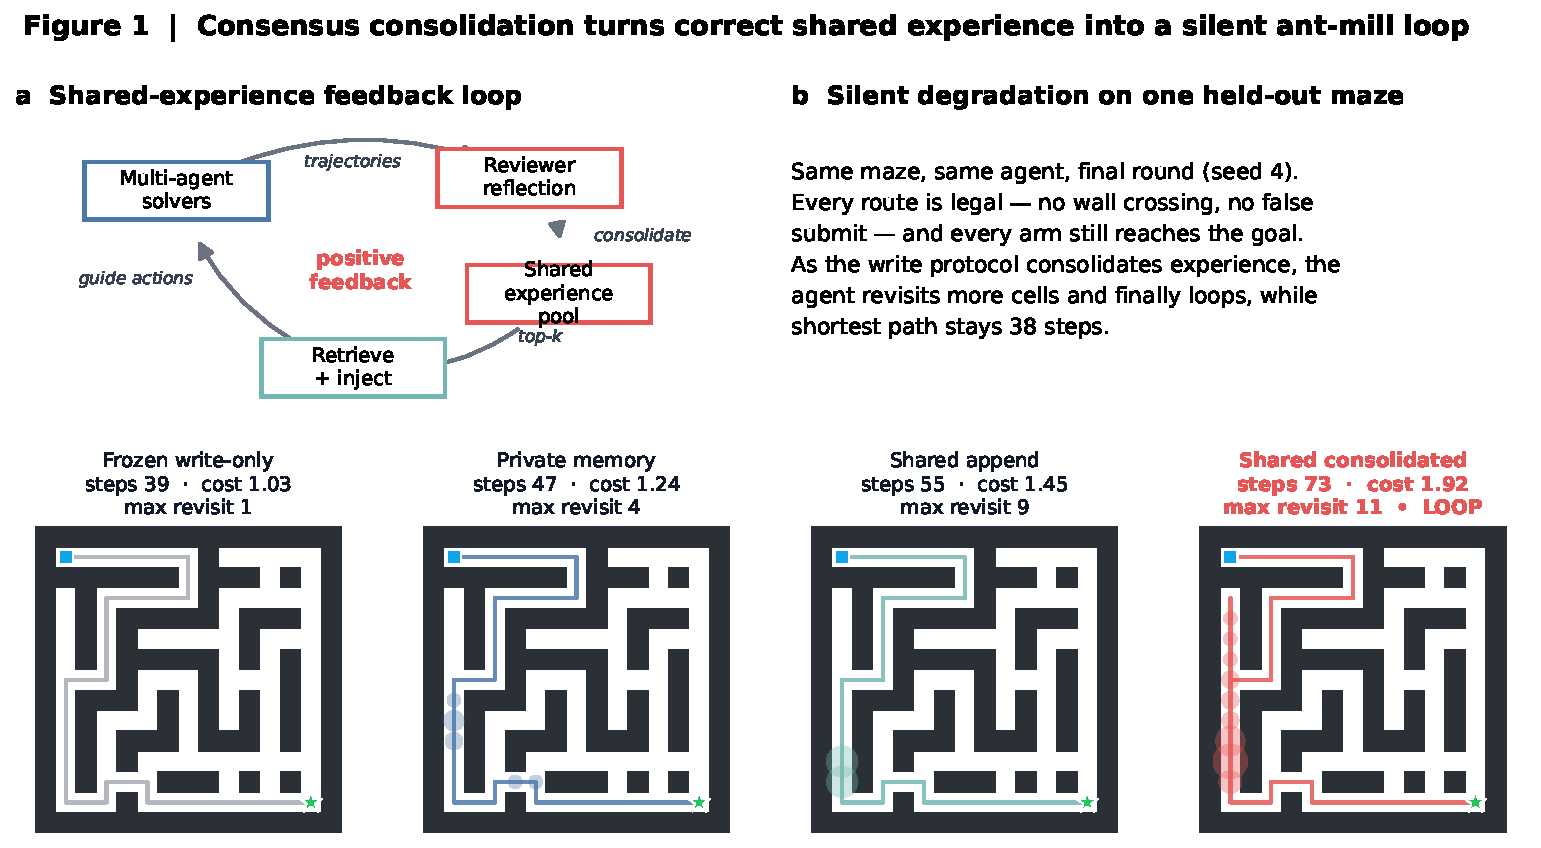
\includegraphics[width=\linewidth]{figure1_mechanism.pdf}
\caption{\textbf{Mechanism microscope and a silent degradation case.}
(a) The shared-experience feedback loop: solver trajectories are reflected into a shared pool,
consolidated by LLM-issued operations, retrieved top-$k$, and injected back as guidance---a
positive-feedback cycle. (b) Same held-out maze and agent, final round; shortest path 38.
Revisit heat (shaded blobs) grows as the write protocol consolidates, culminating in a silent
loop under shared-consolidated memory, while every route stays legal and successful.}
\label{fig:fig1}
\end{figure}

\begin{figure}[p]
\centering
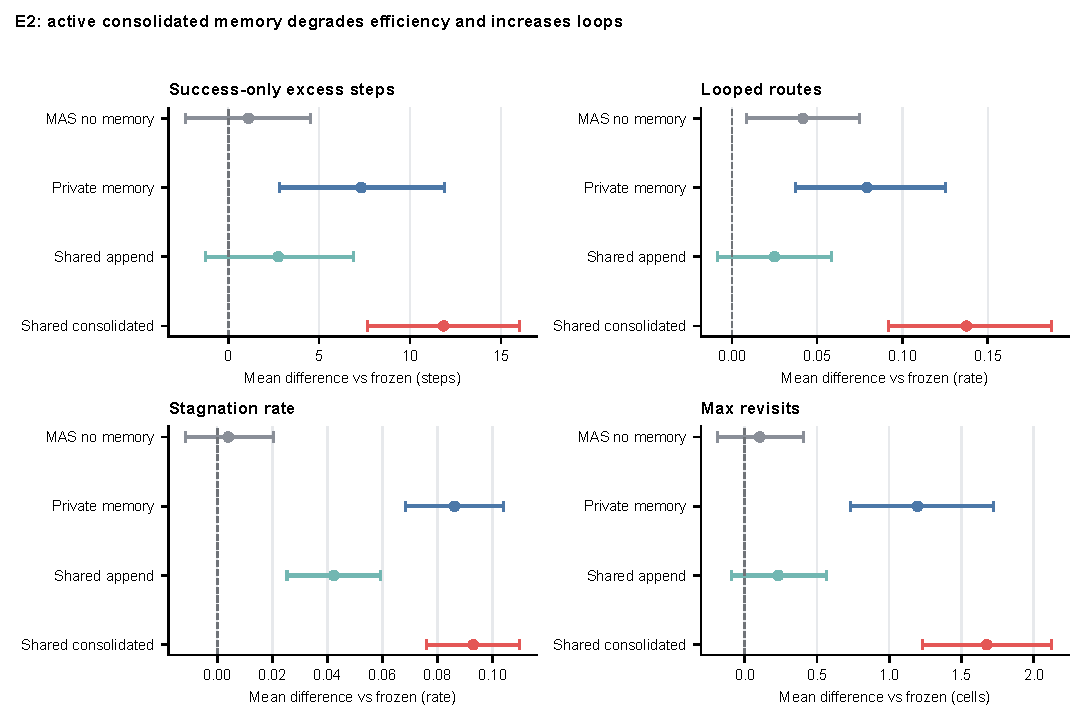
\includegraphics[width=\linewidth]{figure2_e2_main.pdf}
\caption{\textbf{E2 main result: paired differences versus frozen write-only memory}
(five seeds, final round). Points are mean differences; bars are 95\% bootstrap CIs; the dashed
line is zero. Shared-consolidated (red) degrades on all four endpoints with the largest
effects; MAS-no-memory (grey) is on the zero line except for a small loop increase.}
\label{fig:fig2}
\end{figure}

\begin{figure}[p]
\centering
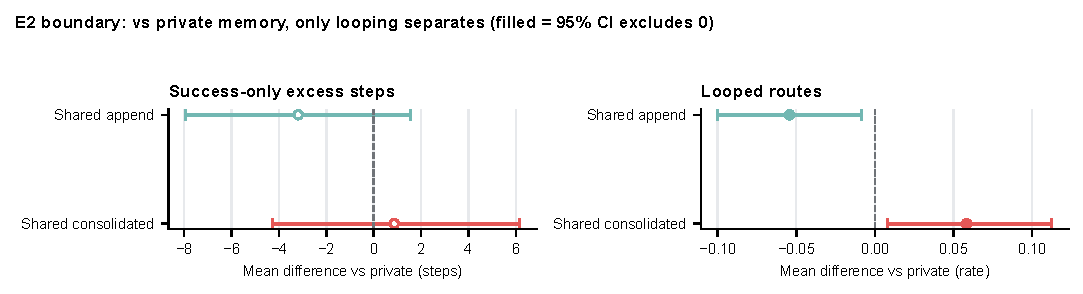
\includegraphics[width=\linewidth]{figure2b_shared_vs_private.pdf}
\caption{\textbf{E2 boundary: shared arms versus a private baseline.}
Filled markers mark CIs that exclude zero. Only looping separates shared-consolidated from
private ($+0.058$, CI $[0.008, 0.113]$); the efficiency contrast does not, and shared-append
actually loops less than private.}
\label{fig:fig2b}
\end{figure}

\begin{figure}[p]
\centering
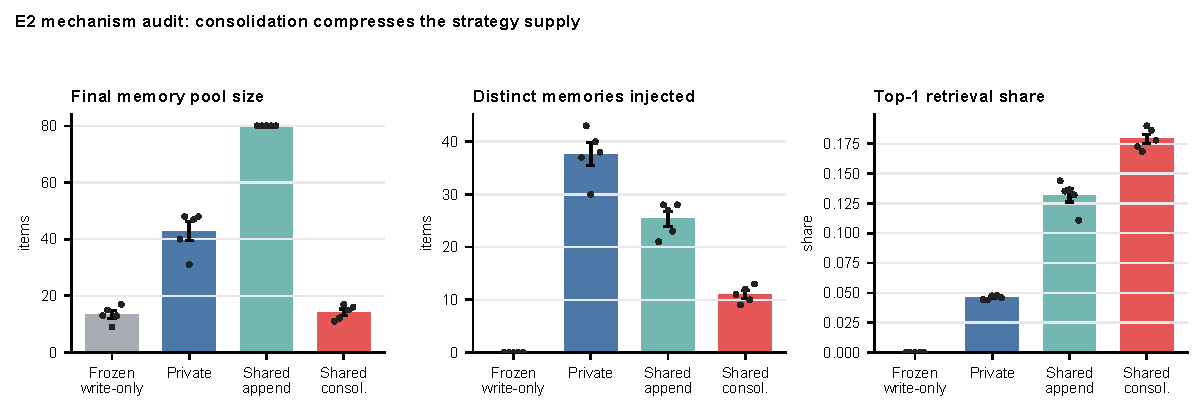
\includegraphics[width=\linewidth]{figure3_write_side_compression.pdf}
\caption{\textbf{Mechanism audit: consolidation compresses the strategy supply.}
Final pool size, distinct experiences ever injected, and top-1 retrieval share across five
seeds (dots). Consensus consolidation keeps a small pool and injects the fewest distinct
strategies, concentrating retrieval; the direct counts (left, centre) carry the claim.
% TODO: add gamma forest plot (DeepSeek vs Qwen per-endpoint CIs) as Figure 5.
}
\label{fig:fig3}
\end{figure}

\end{document}
